\chapter{Análisis de la aplicación}
\label{cap:analisis_aplicacion} 



\section{Especificación de requisitos}
\label{sec:requisitos}
La especificación de requisitos es una etapa clave en el desarrollo de un proyecto, ya que en ella se definen las funcionalidades y condiciones que debe cumplir el sistema. Su objetivo principal
es establecer de manera clara y estructurada las expectativas del producto final.

En esta sección se identifican y detallan los requisitos, tomando en cuenta las necesidades y restricciones detalladas por los 
usuarios y demás partes interesadas. Para ello, es fundamental realizar un análisis que permita comprender qué características son esenciales 
para el correcto funcionamiento del software.

Cada requisito contará con un código único que permitirá clasificarlo y referenciarlo fácilmente a lo largo del documento. Este método de organización facilita su seguimiento y garantiza que 
todas las especificaciones sean consideradas durante el desarrollo del proyecto. 

\subsection{Requisitos funcionales}
\label{subsec:requisitos_funcionales}
Los requisitos funcionales son especificaciones detalladas que describen las funciones y comportamientos que un sistema debe cumplir para 
satisfacer las necesidades del usuario. Estos requisitos definen las acciones que el sistema debe ser capaz de realizar, incluyendo las interacciones
con el usuario y las respuestas a entradas específicas. Estos requisitos son ensenciales para guiar el desarrollo del sistema y asegurar que cumpla con las expectivas del usuario. \cite{pmo2017}

Vamos a clasificar estos requisitos en diferentes grupos según su funcionalidad. 

\begin{itemize}
    \item \textbf{Grupo 1:} Gestión de sesión. En este grupo se incluyen los requisitos relacionados con la autenticación y la gestión de la sesión del usuario.
    \item \textbf{Grupo 2:} Gestión del hogar. En este grupo se incluyen los requisitos relacionados con la creación y gestión de un hogar compartido.
    \item \textbf{Grupo 3:} Gestión de tareas. En este grupo se incluyen los requisitos relacionados con la creación y asignación de tareas en el hogar.
    \item \textbf{Grupo 4:} Gestión de gastos. En este grupo se incluyen los requisitos relacionados con la creación y gestión de gastos en el hogar.
    \item \textbf{Grupo 5:} Gestión de compra. En este grupo se incluyen los requisitos relacionados con la creación y gestión de listas de compra.
\end{itemize}

A continuación, se detallan los requisitos funcionales de cada grupo.

\subsubsection{Grupo 1: Gestión de sesión}
\label{subsubsec:grupo1}


\begin{table}[htb!]
	\centering 
	\begin{tabular}{|p{0.35\linewidth}|p{0.6\linewidth}|}
		\hline
		\rowcolor[HTML]{C0C0C0}  
        \textbf{RF\_01} & \textbf{Registro} \\
		\hline
		\textbf{Prioridad} & Alta \\
		\hline
		\textbf{Descripción} & El sistema debe permitir al usuario registrarse.  \\
		\hline
		\vspace{0.5mm}
		\textbf{Criterios de aceptación} & 
		\begin{minipage}[t]{0.9\linewidth}
			\begin{enumerate}
                \item La pantalla de registro debe pedir el nombre, apellidos, correo electrónico y contraseña
                \item Verificar de que toda la información esté completa.
                \item Comprobar que la información proporcionada sea correcta.
                \item Si hay algún error, mostrar un mensaje de advertencia.
                \item Tras el registro, redirigir al usuario a la pantala de inicio de sesión.
			\end{enumerate}
			\vspace{2mm}
		\end{minipage} \\
		\hline
	\end{tabular}
	\caption{RF\_01}
    \label{req:RF01}
\end{table}

\begin{table}[htb!]
    \begin{tabular}{|p{0.35\linewidth}|p{0.6\linewidth}|}
        \hline
        \rowcolor[HTML]{C0C0C0}  
        \textbf{RF\_02} & \textbf{Inicio de sesión} \\
        \hline
        \textbf{Prioridad} & Alta \\
        \hline
        \textbf{Descripción} & El sistema debe permitir al usuario iniciar sesión.  \\
        \hline
        \vspace{0.5mm}
        \textbf{Criterios de aceptación} & 
        \begin{minipage}[t]{0.9\linewidth}
            \begin{enumerate}
                \item La pantalla de inicio de sesión debe pedir el correo electrónico y contraseña.
                \item Verificar que toda la información esté completa.
                \item Comprobar que la información proporcionada sea correcta.
                \item Si hay algún error, mostrar un mensaje de advertencia.
                \item Tras el inicio de sesión, se redirigirá a la pantalla principal.
            \end{enumerate}
            \vspace{2mm}
        \end{minipage} \\
        \hline
    \end{tabular}
    \caption{RF\_02}
    \label{req:RF02}
\end{table}


\begin{table}[htb!]
    \begin{tabular}{|p{0.35\linewidth}|p{0.6\linewidth}|}
        \hline
        \rowcolor[HTML]{C0C0C0}  
        \textbf{RF\_03} & \textbf{Inicio de sesión con Google} \\
        \hline
        \textbf{Prioridad} & Baja \\
        \hline
        \textbf{Descripción} & El sistema debe permitir al usuario iniciar sesión con Google  \\
        \hline
        \vspace{0.5mm}
        \textbf{Criterios de aceptación} & 
        \begin{minipage}[t]{0.9\linewidth}
            \begin{enumerate}
                \item La pantalla de inicio de sesión debe permitir iniciar sesión con Google.
                \item Si el usuario ya ha iniciado sesión con Google, se redirigirá a la pantalla principal de la aplicación.
                \item Si el usuario no ha iniciado sesión con Google, se registrará automáticamente y se redirigirá a la pantalla principal de la aplicación.
            \end{enumerate}
            \vspace{2mm}
        \end{minipage} \\
        \hline
    \end{tabular}
    \caption{RF\_03}
\end{table}

\begin{table} [htb!]
    \begin{tabular}{|p{0.35\linewidth}|p{0.6\linewidth}|}
        \hline
        \rowcolor[HTML]{C0C0C0}  
        \textbf{RF\_04} & \textbf{Cerrar Sesión} \\
        \hline
        \textbf{Prioridad} & Alta \\
        \hline
        \textbf{Descripción} & El sistema debe permitir al usuario cerrar sesión  \\
        \hline
        \vspace{0.5mm}
        \textbf{Criterios de aceptación} & 
        \begin{minipage}[t]{0.9\linewidth}
            \begin{enumerate}
                \item Debe exitir una opción en la interfaz para cerrar sesión.
                \item Tras cerrar sesión, se redirigirá a la pantalla de bienvenida.
            \end{enumerate}
            \vspace{2mm}
        \end{minipage} \\
        \hline
    \end{tabular}
    \caption{RF\_04}
    \label{req:RF04}

\end{table}


\begin{table}[htb!]
    \begin{tabular}{|p{0.35\linewidth}|p{0.6\linewidth}|}
        \hline
        \rowcolor[HTML]{C0C0C0}  
        \textbf{RF\_05} & \textbf{Ver datos de usuario} \\
        \hline
        \textbf{Prioridad} & Media \\
        \hline
        \textbf{Descripción} & El sistema debe permitir al usuario ver sus datos personales.  \\
        \hline
        \vspace{0.5mm}
        \textbf{Criterios de aceptación} & 
        \begin{minipage}[t]{0.9\linewidth}
            \begin{enumerate}
                \item Debe existir una sección en la interfaz para ver los datos personales del usuario.
                \item El sistema debe mostrar la información del usuario
            \end{enumerate}
            \vspace{2mm}
        \end{minipage} \\
        \hline
    \end{tabular}
    \caption{RF\_05}
    \label{req:RF05}
\end{table}

\begin{table}[htb!]
    \begin{tabular}{|p{0.35\linewidth}|p{0.6\linewidth}|}
        \hline
        \rowcolor[HTML]{C0C0C0}  
        \textbf{RF\_06} & \textbf{Editar datos de usuario} \\
        \hline
        \textbf{Prioridad} & Media \\
        \hline
        \textbf{Descripción} & El sistema debe permitir al usuario editar sus datos personales.  \\
        \hline
        \vspace{0.5mm}
        \textbf{Criterios de aceptación} & 
        \begin{minipage}[t]{0.9\linewidth}
            \begin{enumerate}
                \item Debe existir una opción en la interfaz para editar los datos personales del usuario.
                \item Verificar que los campos obligatorios no estén vacíos y que la información sea válida.
                \item Tras la edición de los datos, se actualizará la información en la base de datos.
            \end{enumerate}
            \vspace{2mm}
        \end{minipage} \\
        \hline
    \end{tabular}
    \label{req:RF06}
    \caption{RF\_06}
\end{table}

\clearpage

\subsubsection{Grupo 2: Gestión del hogar}
\label{subsubsec:grupo2}

\begin{table}[htb!]
    \begin{tabular}{|p{0.35\linewidth}|p{0.6\linewidth}|}
        \hline
        \rowcolor[HTML]{C0C0C0}  
        \textbf{RF\_07} & \textbf{Crear hogar} \\
        \hline
        \textbf{Prioridad} & Alta \\
        \hline
        \textbf{Descripción} & El sistema debe permitir al usuario crear un hogar compartido.  \\
        \hline
        \vspace{0.5mm}
        \textbf{Criterios de aceptación} & 
        \begin{minipage}[t]{0.9\linewidth}
            \begin{enumerate}
                \item Debe exitir una opción en la interfaz para crear un hogar.
                \item El sistema debe pedir el nombre del hogar.
                \item Tras la creación del hogar, se redirigirá a la pantalla principal del hogar.
            \end{enumerate}
            \vspace{2mm}
        \end{minipage} \\
        \hline
    \end{tabular}
    \caption{RF\_07}
    \label{req:RF07}

\end{table}

\begin{table}[htb!]
    \begin{tabular}{|p{0.35\linewidth}|p{0.6\linewidth}|}
        \hline
        \rowcolor[HTML]{C0C0C0}  
        \textbf{RF\_08} & \textbf{Unirse a un hogar} \\
        \hline
        \textbf{Prioridad} & Alta \\
        \hline
        \textbf{Descripción} & El sistema debe permitir al usuario unirse a un hogar compartido.  \\
        \hline
        \vspace{0.5mm}
        \textbf{Criterios de aceptación} & 
        \begin{minipage}[t]{0.9\linewidth}
            \begin{enumerate}
                \item La interfaz de la aplicación debe contener una opción para unirse a un hogar.
                \item El sistema debe pedir el código del hogar.
                \item Verificar que el código del hogar sea válido.
                \item Si la información no es válida , mostrar un mensaje de error.
                \item Tras unirse al hogar, se redirigirá a la pantalla principal del hogar.
            \end{enumerate}
            \vspace{2mm}
        \end{minipage} \\
        \hline
    \end{tabular}
    \caption{RF\_08}
    \label{req:RF08}

\end{table}

\begin{table}[htb!]
    \begin{tabular}{|p{0.35\linewidth}|p{0.6\linewidth}|}
        \hline
        \rowcolor[HTML]{C0C0C0}  
        \textbf{RF\_09} & \textbf{Abandonar hogar} \\
        \hline
        \textbf{Prioridad} & Alta \\
        \hline
        \textbf{Descripción} & El sistema debe permitir al usuario abandonar un hogar compartido.  \\
        \hline
        \vspace{0.5mm}
        \textbf{Criterios de aceptación} & 
        \begin{minipage}[t]{0.9\linewidth}
            \begin{enumerate}
                \item La interfaz de la aplicación debe contener una opción para abandonar el hogar.
                \item Si el usuario confirma, abandonará el hogar y se redirigirá a la pantalla principal de la aplicación.
            \end{enumerate}
            \vspace{2mm}
        \end{minipage} \\
        \hline
    \end{tabular}
    \caption{RF\_09}
    \label{req:RF09}

\end{table}

\begin{table}[htb!]
    \begin{tabular}{|p{0.35\linewidth}|p{0.6\linewidth}|}
        \hline
        \rowcolor[HTML]{C0C0C0}  
        \textbf{RF\_10} & \textbf{Ver datos del hogar} \\
        \hline
        \textbf{Prioridad} & Alta \\
        \hline
        \textbf{Descripción} & El sistema debe permitir al usuario ver los datos del hogar.  \\
        \hline
        \vspace{0.5mm}
        \textbf{Criterios de aceptación} & 
        \begin{minipage}[t]{0.9\linewidth}
            \begin{enumerate}
                \item Debe existir una sección en la interfaz para ver los datos del hogar.
                \item Al acceder a la sección, se mostrará la información del hogar.
            \end{enumerate}
            \vspace{2mm}
        \end{minipage} \\
        \hline
    \end{tabular}
    \caption{RF\_10}
    \label{req:RF10}
\end{table}

\begin{table}[htb!]
    \begin{tabular}{|p{0.35\linewidth}|p{0.6\linewidth}|}
        \hline
        \rowcolor[HTML]{C0C0C0}  
        \textbf{RF\_11} & \textbf{Editar hogar} \\ 
        \hline
        \textbf{Prioridad} & Alta \\ 
        \hline
        \textbf{Descripción} & El sistema debe permitir al usuario editar los datos del hogar. \\ 
        \hline
        \vspace{0.5mm}
        \textbf{Criterios de aceptación} & 
        \begin{minipage}[t]{0.9\linewidth}
            \begin{enumerate}
                \item Debe existir una opción en la interfaz para editar los datos del hogar.
                \item Verificar que los campos obligatorios no estén vacios y que la información sea válida.
                \item Si los campos no son válidos, mostrar un mensaje de error.
                \item Tras la edición de los datos, se actualizará la información en la base de datos.
            \end{enumerate}
            \vspace{2mm}
        \end{minipage} \\ 
        \hline
    \end{tabular}
    \caption{RF\_11}
    \label{req:RF11}
\end{table}


\clearpage

\subsubsection{Grupo 3: Gestión de tareas}
\label{subsubsec:grupo3}

\begin{table}[htb!]
    \begin{tabular}{|p{0.35\linewidth}|p{0.6\linewidth}|}
        \hline
        \rowcolor[HTML]{C0C0C0}  
        \textbf{RF\_12} & \textbf{Crear tarea} \\
        \hline
        \textbf{Prioridad} & Alta \\
        \hline
        \textbf{Descripción} & El sistema debe permitir al usuario crear una tarea.  \\
        \hline
        \vspace{0.5mm}
        \textbf{Criterios de aceptación} & 
        \begin{minipage}[t]{0.9\linewidth}
            \begin{enumerate}
                \item La interfaz de la aplicación debe contener una opción para crear una tarea.
                \item El sistema nos pedirá la información de la tarea.
                \item Verificar que los campos  obligatorios no estén vacíos y que la información ssea válida.
                \item Si la información no es válida, mostrar un mensaje de error.
            \end{enumerate}
            \vspace{2mm}
        \end{minipage} \\
        \hline
    \end{tabular}
    \caption{RF\_12}
    \label{req:RF12}
\end{table}


\begin{table}[htb!]
    \begin{tabular}{|p{0.35\linewidth}|p{0.6\linewidth}|}
        \hline
        \rowcolor[HTML]{C0C0C0}  
        \textbf{RF\_13} & \textbf{Consultar planificación semanal} \\
        \hline
        \textbf{Prioridad} & Alta \\
        \hline
        \textbf{Descripción} & El sistema debe permitir al usuario poder consultar las tareas asignadas por semanas.  \\
        \hline
        \vspace{0.5mm}
        \textbf{Criterios de aceptación} & 
        \begin{minipage}[t]{0.9\linewidth}
            \begin{enumerate}
                \item Debe existir una sección en la interfaz para consultar la planificación semanal.
                \item Al acceder a la sección, se mostrarán las tareas asignadas por semanas.
                \item Si no hay tareas asignadas, mostrar un mensaje indicando que no hay tareas asignadas.
            \end{enumerate}
            \vspace{2mm}
        \end{minipage} \\
        \hline
    \end{tabular}
    \caption{RF\_13}
    \label{req:RF13}
\end{table}

\begin{table}[htb!]
    \begin{tabular}{|p{0.35\linewidth}|p{0.6\linewidth}|}
        \hline
        \rowcolor[HTML]{C0C0C0}  
        \textbf{RF\_14} & \textbf{Marcar tarea como realizada} \\
        \hline
        \textbf{Prioridad} & Alta \\
        \hline
        \textbf{Descripción} & El sistema debe permitir al usuario poder marcar una tarea como realizada.  \\
        \hline
        \vspace{0.5mm}
        \textbf{Criterios de aceptación} & 
        \begin{minipage}[t]{0.9\linewidth}
            \begin{enumerate}
                \item Debe existir una opción en la interfaz para marcar una tarea como realizada.
                \item Si el usuario confirma, la tarea se marcará como realizada y se actualizará la información en la base de datos.
            \end{enumerate}
            \vspace{2mm}
        \end{minipage} \\
        \hline
    \end{tabular}
    \caption{RF\_14}
    \label{req:RF14}
\end{table}

\begin{table}[htb!]
    \begin{tabular}{|p{0.35\linewidth}|p{0.6\linewidth}|}
        \hline
        \rowcolor[HTML]{C0C0C0}  
        \textbf{RF\_15} & \textbf{Editar Tarea} \\
        \hline
        \textbf{Prioridad} & Alta \\
        \hline
        \textbf{Descripción} & El sistema debe permitir al usuario poder modificar una tarea.  \\
        \hline
        \vspace{0.5mm}
        \textbf{Criterios de aceptación} & 
        \begin{minipage}[t]{0.9\linewidth}
            \begin{enumerate}
                \item Debe existir una opción en la interfaz para modificar una tarea.
                \item Verificar que los campos obligatorios no estén vacíos y que la información sea válida.
                \item Si los campos no son válidos, mostrar un mensaje de error.
                \item Tras la modificación de la tarea, se actualizará la información en la base de datos.
            \end{enumerate}
            \vspace{2mm}
        \end{minipage} \\
        \hline
    \end{tabular}
    \caption{RF\_15}
    \label{req:RF15}
\end{table}

\begin{table}[htb!]
    \begin{tabular}{|p{0.35\linewidth}|p{0.6\linewidth}|}
        \hline
        \rowcolor[HTML]{C0C0C0}  
        \textbf{RF\_16} & \textbf{Eliminar Tarea} \\
        \hline
        \textbf{Prioridad} & Alta \\
        \hline
        \textbf{Descripción} & El sistema debe permitir al usuario poder eliminar una tarea.  \\
        \hline
        \vspace{0.5mm}
        \textbf{Criterios de aceptación} & 
        \begin{minipage}[t]{0.9\linewidth}
            \begin{enumerate}
                \item Debe existir una opción en la interfaz para eliminar una tarea.
                \item Si el usuario confirma, la tarea se eliminará y se actualizará la información en la base de datos.
            \end{enumerate}
            \vspace{2mm}
        \end{minipage} \\
        \hline
    \end{tabular}
    \caption{RF\_16}
    \label{req:RF16}
\end{table}

\begin{table}[htb!]
    \begin{tabular}{|p{0.35\linewidth}|p{0.6\linewidth}|}
        \hline
        \rowcolor[HTML]{C0C0C0}  
        \textbf{RF\_17} & \textbf{Ver datos de una tarea} \\
        \hline
        \textbf{Prioridad} & Alta \\
        \hline
        \textbf{Descripción} & El sistema debe permitir al usuario ver los datos de una tarea.  \\
        \hline
        \vspace{0.5mm}
        \textbf{Criterios de aceptación} & 
        \begin{minipage}[t]{0.9\linewidth}
            \begin{enumerate}
                \item Debe existir una sección en la interfaz para ver los datos de una tarea.
                \item Al acceder a la sección, se mostrarán los datos de la tarea.
            \end{enumerate}
            \vspace{2mm}
        \end{minipage} \\
        \hline
    \end{tabular}
    \caption{RF\_17}
    \label{req:RF17}
\end{table}

\begin{table}[htb!]
    \begin{tabular}{|p{0.35\linewidth}|p{0.6\linewidth}|}
        \hline
        \rowcolor[HTML]{C0C0C0}  
        \textbf{RF\_18} & \textbf{Ver calendario de tareas} \\
        \hline
        \textbf{Prioridad} & Alta \\
        \hline
        \textbf{Descripción} & El sistema debe permitir al usuario ver el calendario de tareas.  \\
        \hline
        \vspace{0.5mm}
        \textbf{Criterios de aceptación} & 
        \begin{minipage}[t]{0.9\linewidth}
            \begin{enumerate}
                \item La interfaz de la aplicación debe contener una sección para ver el calendario de tareas.
                \item Al acceder a la sección, se mostrará un calendario con las tareas asignadas.
            \end{enumerate}
            \vspace{2mm}
        \end{minipage} \\
        \hline
    \end{tabular}
    \caption{RF\_18}
    \label{req:RF18}
\end{table}



\clearpage

\subsubsection{Grupo 4: Gestión de gastos}
\label{subsubsec:grupo4}

\begin{table}[htb!]
    \begin{tabular}{|p{0.35\linewidth}|p{0.6\linewidth}|}
        \hline
        \rowcolor[HTML]{C0C0C0}  
        \textbf{RF\_19} & \textbf{Crear gasto} \\
        \hline
        \textbf{Prioridad} & Alta \\
        \hline
        \textbf{Descripción} & El sistema debe permitir al usuario crear un gasto.  \\
        \hline
        \vspace{0.5mm}
        \textbf{Criterios de aceptación} & 
        \begin{minipage}[t]{0.9\linewidth}
            \begin{enumerate}
                \item Debe existir una opción en la interfaz para crear un gasto.
                \item El sistema debe pedir la información del gasto.
                \item Verificar que los campos obligatorios no estén vacíos y que la información sea válida.
                \item El sistema debe recalcular las deudas pendientes.
            \end{enumerate}
            \vspace{2mm}
        \end{minipage} \\
        \hline
    \end{tabular}
    \caption{RF\_19}
    \label{req:RF19}
\end{table}

\begin{table}[htb!]
    \begin{tabular}{|p{0.35\linewidth}|p{0.6\linewidth}|}
        \hline
        \rowcolor[HTML]{C0C0C0}  
        \textbf{RF\_20} & \textbf{Editar gasto} \\
        \hline
        \textbf{Prioridad} & Alta \\
        \hline
        \textbf{Descripción} & El sistema debe permitir al usuario modificar un gasto.  \\
        \hline
        \vspace{0.5mm}
        \textbf{Criterios de aceptación} & 
        \begin{minipage}[t]{0.9\linewidth}
            \begin{enumerate}
                \item Deber existir una opción en la interfaz para modificar un gasto.
                \item El sistema debe pedir la información del gasto.
                \item Verificar que los campos obligatorios no estén vacíos y que la información sea válida.
                \item Tras la modificación del gasto, se actualizará la información en la base de datos.
                \item El sistema debe recalcular las deudas pendientes.
            \end{enumerate}
            \vspace{2mm}
        \end{minipage} \\
        \hline
    \end{tabular}
    \caption{RF\_20}
    \label{req:RF20}
\end{table}

\begin{table}[htb!]
    \begin{tabular}{|p{0.35\linewidth}|p{0.6\linewidth}|}
        \hline
        \rowcolor[HTML]{C0C0C0}  
        \textbf{RF\_21} & \textbf{Eliminar gasto} \\
        \hline
        \textbf{Prioridad} & Alta \\
        \hline
        \textbf{Descripción} & El sistema debe permitir al usuario eliminar un gasto.  \\
        \hline
        \vspace{0.5mm}
        \textbf{Criterios de aceptación} & 
        \begin{minipage}[t]{0.9\linewidth}
            \begin{enumerate}
                \item Debe existir una opción en la interfaz para eliminar un gasto.
                \item Si el usuario confirma, el gasto se eliminará y se actualizará la información en la base de datos.
                \item El sistema debe recalcular las deudas pendientes.
            \end{enumerate}
            \vspace{2mm}
        \end{minipage} \\
        \hline
    \end{tabular}
    \caption{RF\_21}
    \label{req:RF21}
\end{table}

\begin{table}[htb!]
    \begin{tabular}{|p{0.35\linewidth}|p{0.6\linewidth}|}
        \hline
        \rowcolor[HTML]{C0C0C0}  
        \textbf{RF\_22} & \textbf{Saldar deuda} \\
        \hline
        \textbf{Prioridad} & Alta \\
        \hline
        \textbf{Descripción} & El sistema debe permitir al usuario saldar una deuda.  \\
        \hline
        \vspace{0.5mm}
        \textbf{Criterios de aceptación} & 
        \begin{minipage}[t]{0.9\linewidth}
            \begin{enumerate}
                \item Debe existir una opción en la interfaz para saldar una deuda.
                \item Si el usuario confirma, la deuda se marcará como saldada y se actualizará la información en la base de datos.
            \end{enumerate}
            \vspace{2mm}
        \end{minipage} \\
        \hline
    \end{tabular}
    \caption{RF\_22}
    \label{req:RF22}
\end{table}

\begin{table}[htb!]
    \begin{tabular}{|p{0.35\linewidth}|p{0.6\linewidth}|}
        \hline
        \rowcolor[HTML]{C0C0C0}  
        \textbf{RF\_23} & \textbf{Ver deudas} \\
        \hline
        \textbf{Prioridad} & Alta \\
        \hline
        \textbf{Descripción} & El sistema debe permitir al usuario ver las deudas pendientes.  \\
        \hline
        \vspace{0.5mm}
        \textbf{Criterios de aceptación} & 
        \begin{minipage}[t]{0.9\linewidth}
            \begin{enumerate}
                \item Debe existir una sección en la interfaz para ver las deudas pendientes.
                \item Al acceder a la sección, se mostrarán las deudas pendientes.
                \item Si no hay deudas pendientes, mostrar un mensaje indicando que no hay deudas pendientes.
            \end{enumerate}
            \vspace{2mm}
        \end{minipage} \\
        \hline
    \end{tabular}
    \caption{RF\_23}
    \label{req:RF23}
\end{table}

\begin{table}[htb!]
    \begin{tabular}{|p{0.35\linewidth}|p{0.6\linewidth}|}
        \hline
        \rowcolor[HTML]{C0C0C0}  
        \textbf{RF\_24} & \textbf{Ver detalles de un gasto} \\
        \hline
        \textbf{Prioridad} & Alta \\
        \hline
        \textbf{Descripción} & El sistema debe permitir al usuario ver los detalles de un gasto.  \\
        \hline
        \vspace{0.5mm}
        \textbf{Criterios de aceptación} & 
        \begin{minipage}[t]{0.9\linewidth}
            \begin{enumerate}
                \item La interfaz de la aplicación debe contener una sección para ver los detalles de un gasto.
                \item Al acceder a la sección, se mostrarán los detalles del gasto.
                \item Si no hay datos disponibles, mostrar un mensaje indicando que no hay datos disponibles.
            \end{enumerate}
            \vspace{2mm}
        \end{minipage} \\
        \hline
    \end{tabular}
    \caption{RF\_24}
    \label{req:RF24}
\end{table}
\clearpage




\subsubsection{Grupo 5: Gestión de compra}
\label{subsubsec:grupo5}

\begin{table}[htb!]
    \begin{tabular}{|p{0.35\linewidth}|p{0.6\linewidth}|}
        \hline
        \rowcolor[HTML]{C0C0C0}  
        \textbf{RF\_25} & \textbf{Crear lista de la compra} \\ 
        \hline
        \textbf{Prioridad} & Alta \\ 
        \hline
        \textbf{Descripción} & El sistema debe permitir al usuario crear una lista de la compra. \\ 
        \hline
        \vspace{0.5mm}
        \textbf{Criterios de aceptación} & 
        \begin{minipage}[t]{0.9\linewidth}
            \begin{enumerate}
                \item Debe existir una opción en la interfaz para crear una lista de la compra.
                \item El sistema debe pedir el nombre de la lista de la compra.
            \end{enumerate}
            \vspace{2mm}
        \end{minipage} \\ 
        \hline
    \end{tabular}
    \caption{RF\_25}
    \label{req:RF25}
\end{table}

\begin{table}[htb!]
    \begin{tabular}{|p{0.35\linewidth}|p{0.6\linewidth}|}
        \hline
        \rowcolor[HTML]{C0C0C0}  
        \textbf{RF\_26} & \textbf{Añadir producto a la lista de la compra} \\ 
        \hline
        \textbf{Prioridad} & Alta \\ 
        \hline
        \textbf{Descripción} & El sistema debe permitir al usuario añadir un producto a la lista de la compra. \\ 
        \hline
        \vspace{0.5mm}
        \textbf{Criterios de aceptación} & 
        \begin{minipage}[t]{0.9\linewidth}
            \begin{enumerate}
                \item Debe existir una opción en la interfaz para añadir un producto a la lista de la compra.
                \item El sistema debe la información del producto.
                \item Verificar que los campos obligatorios no estén vacíos.
                \item Tras añadir el producto, se actualizará la lista de la compra. 
            \end{enumerate}
            \vspace{2mm}
        \end{minipage} \\ 
        \hline
    \end{tabular}
    \caption{RF\_26}
    \label{req:RF26}
\end{table}

\begin{table}[htb!]
    \begin{tabular}{|p{0.35\linewidth}|p{0.6\linewidth}|}
        \hline
        \rowcolor[HTML]{C0C0C0}  
        \textbf{RF\_27} & \textbf{Eliminar producto de la lista de la compra} \\ 
        \hline
        \textbf{Prioridad} & Alta \\ 
        \hline
        \textbf{Descripción} & El sistema debe permitir al usuario eliminar un producto de la lista de la compra. \\ 
        \hline
        \vspace{0.5mm}
        \textbf{Criterios de aceptación} & 
        \begin{minipage}[t]{0.9\linewidth}
            \begin{enumerate}
                \item Debe existir una opción en la interfaz para eliminar un producto de la lista de la compra.
                \item Si el usuario confirma, el producto se eliminará de la lista de la compra y se actualizará la información en la base de datos.
            \end{enumerate}
            \vspace{2mm}
        \end{minipage} \\ 
        \hline
    \end{tabular}
    \caption{RF\_27}
    \label{req:RF27}
\end{table}

\begin{table}[htb!]
    \begin{tabular}{|p{0.35\linewidth}|p{0.6\linewidth}|}
        \hline
        \rowcolor[HTML]{C0C0C0}  
        \textbf{RF\_28} & \textbf{Eliminar lista de la compra} \\ 
        \hline
        \textbf{Prioridad} & Alta \\ 
        \hline
        \textbf{Descripción} & El sistema debe permitir al usuario eliminar una lista de la compra. \\ 
        \hline
        \vspace{0.5mm}
        \textbf{Criterios de aceptación} & 
        \begin{minipage}[t]{0.9\linewidth}
            \begin{enumerate}
                \item Debe existir una opción en la interfaz para eliminar una lista de la compra.
                \item Si el usuario confirma, la lista de la compra se eliminará y los productos asociados a ella  y se actualizará la información en la base de datos.
            \end{enumerate}
            \vspace{2mm}
        \end{minipage} \\ 
        \hline
    \end{tabular}
    \caption{RF\_28}
    \label{req:RF28}
\end{table}

\begin{table}[htb!]
    \begin{tabular}{|p{0.35\linewidth}|p{0.6\linewidth}|}
        \hline
        \rowcolor[HTML]{C0C0C0}  
        \textbf{RF\_29} & \textbf{Ver productos de la lista de la compra} \\ 
        \hline
        \textbf{Prioridad} & Alta \\ 
        \hline
        \textbf{Descripción} & El sistema debe permitir al usuario ver los productos de una lista de la compra. \\ 
        \hline
        \vspace{0.5mm}
        \textbf{Criterios de aceptación} & 
        \begin{minipage}[t]{0.9\linewidth}
            \begin{enumerate}
                \item Debe existir una sección en la interfaz para ver los productos de la lista de la compra.
                \item Al acceder a la sección, se mostrarán los productos de la lista de la compra.
                \item Si no hay productos en la lista, mostrar un mensaje indicando que no hay productos en la lista.
            \end{enumerate}
            \vspace{2mm}
        \end{minipage} \\ 
        \hline
    \end{tabular}
    \caption{RF\_29}
    \label{req:RF29}
\end{table}

\begin{table}[htb!]
    \begin{tabular}{|p{0.35\linewidth}|p{0.6\linewidth}|}
        \hline
        \rowcolor[HTML]{C0C0C0}  
        \textbf{RF\_30} & \textbf{Editar producto de la lista de la compra} \\ 
        \hline
        \textbf{Prioridad} & Alta \\ 
        \hline
        \textbf{Descripción} & El sistema debe permitir al usuario editar un producto de la lista de la compra. \\ 
        \hline
        \vspace{0.5mm}
        \textbf{Criterios de aceptación} & 
        \begin{minipage}[t]{0.9\linewidth}
            \begin{enumerate}
                \item Debe existir una opción en la interfaz para editar un producto de la lista de la compra.
                \item Verificar que los campos obligatorios no estén vacíos y que la información sea válida.
                \item Tras la edición del producto, se actualizará la lista de la compra.
            \end{enumerate}
            \vspace{2mm}
        \end{minipage} \\ 
        \hline
    \end{tabular}
    \caption{RF\_30}
    \label{req:RF30}
\end{table}


\clearpage

\subsection{Requisitos no funcionales}

Los \textbf{requisitos no funcionales} son aquellos que describen las características y restricciones del sistema, pero no están 
directamentes relacionadas con sus funcionalidades. En lugar de especificar qué hace el sistema, establecen cómo debe hacerlo.
Estos requisitos garantizan la calidad, el rendimiento, la seguridad, la usabilidad y otros aspectos clave del software. \cite{sommerville2015}.

\begin{table}[htb!]
    \begin{tabular}{|p{0.35\linewidth}|p{0.6\linewidth}|}
        \hline
        \rowcolor[HTML]{C0C0C0}
        \textbf{RNF\_01} & \textbf{Seguridad} \\
        \hline
        \textbf{Prioridad} & Alta \\
        \hline
        \textbf{Descripción} & 
        El sistema protegerá los datos de los usuarios mediante autenticación con Firebase Authentication, 
        reglas de seguridad en Firestore y cifrado en la comunicación de datos. \\
        \hline
    \end{tabular}
    \caption{RNF\_01}
\end{table}


\begin{table}[htb!]
    \begin{tabular}{|p{0.35\linewidth}|p{0.6\linewidth}|}
        \hline
        \rowcolor[HTML]{C0C0C0}
        \textbf{RNF\_02} & \textbf{Usabilidad} \\
        \hline
        \textbf{Prioridad} & Alta \\
        \hline
        \textbf{Descripción} & 
        El sistema debe ser fácil de usar y comprender para los usuarios. 
        Para ello, se implementará una interfaz intuitiva con una navegación clara y un diseño consistente. 
        Además, se realizarán pruebas con usuarios reales para identificar mejoras en la experiencia de uso. \\
        \hline
    \end{tabular}
    \caption{RNF\_02}
\end{table}


\begin{table}[htb!]
    \begin{tabular}{|p{0.35\linewidth}|p{0.6\linewidth}|}
        \hline
        \rowcolor[HTML]{C0C0C0}
        \textbf{RNF\_03} & \textbf{Rendimiento} \\
        \hline
        \textbf{Prioridad} & Bajo \\
        \hline
        \textbf{Descripción} & 
        El sistema optimizará el rendimiento mediante consultas eficientes en Firestore y una interfaz ligera para mejorar la velocidad de respuesta. \\
        \hline
    \end{tabular}
    \caption{RNF\_03}
\end{table}



\begin{table}[htb!]
    \begin{tabular}{|p{0.35\linewidth}|p{0.6\linewidth}|}
        \hline
        \rowcolor[HTML]{C0C0C0}
        \textbf{RNF\_04} & \textbf{Compatibilidad} \\
        \hline
        \textbf{Prioridad} & Media \\
        \hline
        \textbf{Descripción} & El software debe estar disponible para diferentes sistemas operativos (iOS, Android). \\
        \hline
    \end{tabular}
    \caption{RNF\_04}
\end{table}

\begin{table}[htb!]
    \begin{tabular}{|p{0.35\linewidth}|p{0.6\linewidth}|}
        \hline
        \rowcolor[HTML]{C0C0C0}
        \textbf{RNF\_05} & \textbf{Accesibilidad} \\
        \hline
        \textbf{Prioridad} & Baja \\
        \hline
        \textbf{Descripción} & 
        El sistema implementará etiquetas accesibles y un diseño con buen contraste para mejorar la usabilidad para personas con discapacidades. \\
        \hline
    \end{tabular}
    \caption{RNF\_05}
\end{table}


\clearpage

\section{Modelos de casos de uso}
\label{sec:modelos-casos-uso}

Los modelos de de casos de uso nos permiten representar las iteracciones entre los usuarios y el sistema de forma clara. En este apartado, se presentan los casos de uso de la aplicación 
que reflejan las principales funcionalidades que la aplicación va a ofrecer. 

Cada caso de uso describe una funcionalidad específica, estableciendo los actores involucrados. En este caso los actores son: 

\begin{itemize}
    \item \textbf{Usuario}: La persona que utiliza la aplicación. 
    \item \textbf{Administrador}: La persona que gestiona la aplicación y la base de datos. 
\end{itemize}


\subsection{Diagrama de casos de uso}

A continuación, se muestran los diagramas de casos de uso, que se han dividido en paquetes (cada paquete corresponde a un grupo de funcionales que ya establecimos en el apartado de requisitos funcionales)
y así poder representar de forma más clara las funcionalidades de la aplicación.


\begin{figure}[htb!]
    \centering
    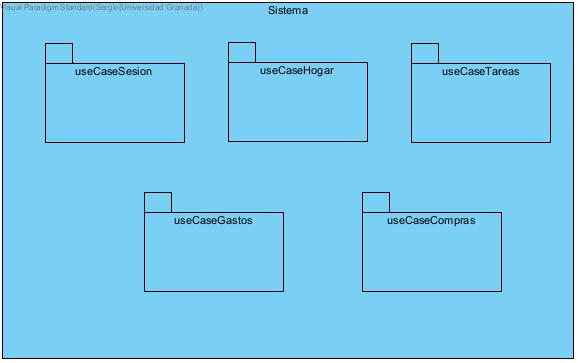
\includegraphics[width=\textwidth]{../capitulos/img/diagrama_paquetes.jpg}
    \caption{Diagrama de paquetes de casos de uso}
    \label{fig:diagrama_paquetes_casos_uso}
\end{figure}


\begin{figure}[htb!]
    \centering
    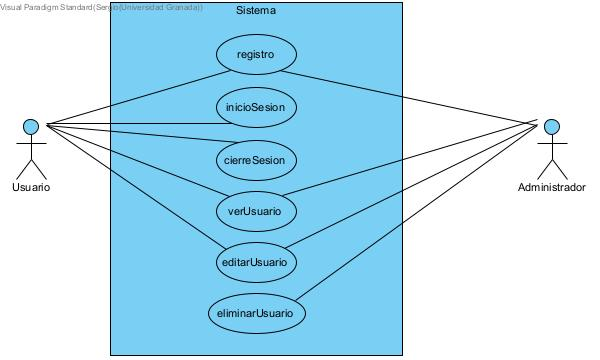
\includegraphics[width=\textwidth]{../capitulos/img/diagrama_sesion.jpg}
    \caption{Diagrama de casos de uso de la gestión de sesión}
    \label{fig:diagrama_sesion_casos_uso}
\end{figure}

\begin{figure}[htb!]
    \centering
    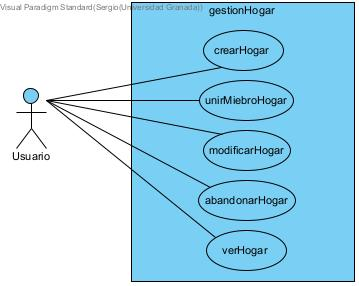
\includegraphics[width=\textwidth]{../capitulos/img/diagrama_hogar.jpg}
    \caption{Diagrama de casos de uso de la gestion de hogar}
    \label{fig:diagrama_hogar_casos_uso}
\end{figure}

\begin{figure}[htb!]
    \centering
    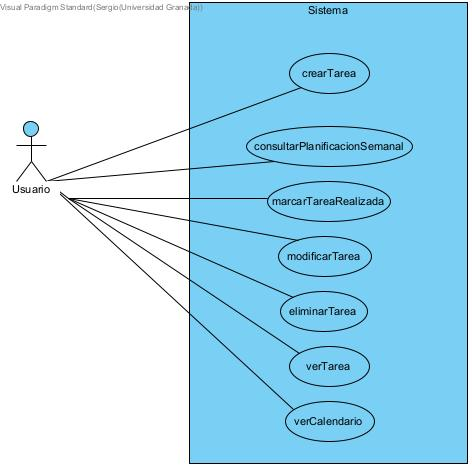
\includegraphics[width=\textwidth]{../capitulos/img/diagrama_tareas.jpg}
    \caption{Diagrama de casos de uso de la gestion de tareas}
    \label{fig:diagrama_tareas_casos_uso}
\end{figure}


\begin{figure}[htb!]
    \centering
    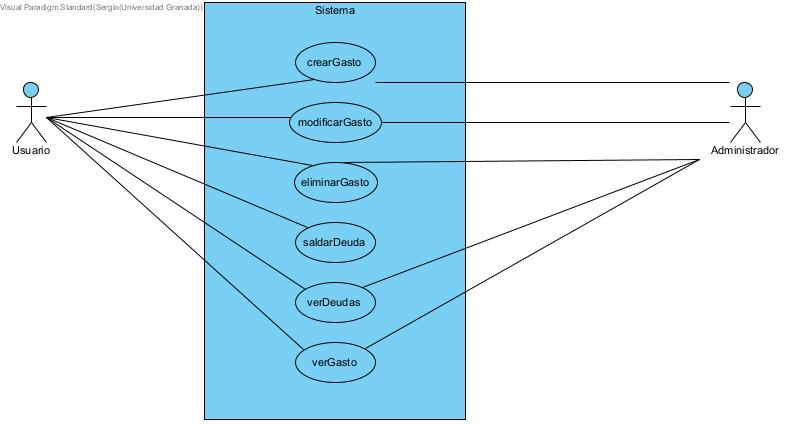
\includegraphics[width=\textwidth]{../capitulos/img/diagrama_gastos.jpg}
    \caption{Diagrama de casos de uso de la gestion de gastos}
    \label{fig:diagrama_gastos_casos_uso}
\end{figure}


\begin{figure}[htb!]
    \centering
    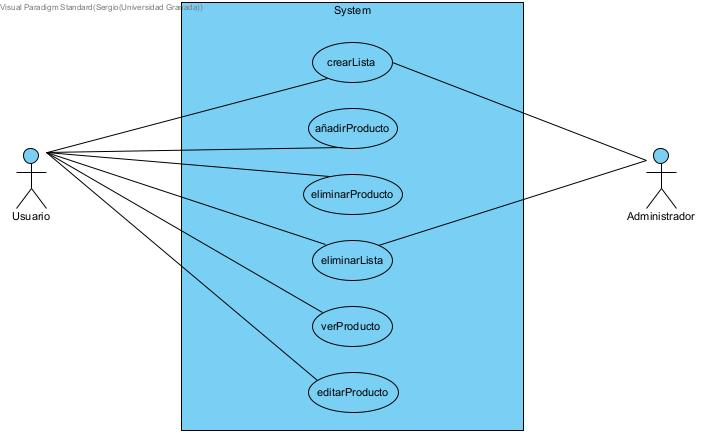
\includegraphics[width=\textwidth]{../capitulos/img/diagrama_compra.jpg}
    \caption{Diagrama de casos de uso de la gestion de compra}
    \label{fig:diagrama_compra_casos_uso}
\end{figure}

\clearpage

\subsection{Descripción de los casos de uso}

En esta sección se describen los casos de uso de la aplicación, indicando los actores involucrados, 
la descripción y los pasos a seguir para llevar a cabo la funcionalidad.



\begin{table}[H]
	\centering
	\begin{tabular}{| m{0.2\textwidth} | m{0.2\textwidth} | m{0.2\textwidth} | m{0.2\textwidth} |}
		\hline
		\rowcolor[HTML]{C0C0C0} Caso de Uso & \multicolumn{2}{|m{0.43\textwidth}|}{registro} &  CU1\\ 
		\hline
		Actores & \multicolumn{3}{l|}{Usuario, Administrador} \\ 
		\hline
		Tipo & \multicolumn{3}{l|}{Obligatorio} \\ 
		\hline
		Referencias & \multicolumn{3}{l|}{\hyperref[req:RF01]{RF\_01}} \\ 
		\hline
		Precondición & \multicolumn{3}{l|}{El usuario no debe estar registrado en el sistema.} \\ 
		\hline
        Postcondición & \multicolumn{3}{l|}{El usuario queda registrado en el sistema.} \\ 
		\hline
		Autor & \multicolumn{3}{l|}{Sergio Muñoz} \\ 
		\hline
		Fecha & 28/02/2025 & Versión & 1.0 \\
		\hline
	\end{tabular}
\end{table}

\begin{table}[H]
	\centering
	\begin{tabular}{| m{0.2\textwidth} | m{0.2\textwidth} | m{0.2\textwidth} | m{0.2\textwidth} |}
		\hline
		Propósito & \multicolumn{3}{m{0.67\textwidth}|}{El usuario debe ser capaz de crearse una cuenta en el sistema.}   \\ 
		\hline
		Resumen & \multicolumn{3}{m{0.67\textwidth}|}{El usuario introduce los datos necesarios para crear una cuenta.} \\ 
		\hline
	\end{tabular}
\end{table}

\begin{table}[H]
	\centering
	\begin{tabular}{| m{0.03\textwidth} | m{0.37\textwidth} | m{0.03\textwidth} | m{0.37\textwidth} |}
		\hline
		\multicolumn{4}{|m{0.9\textwidth}|}{Curso normal}     \\ 
		\hline
		1. & Usuario: Introduce su nombre, apellidos, correo electrónico y contraseña. 
        & 2. & El sistema verifica que los campos no estén vacíos y que la información introducida sea válida. \\ 
		\hline
		3. & Usuario: Confirma el registro. & 4. & El sistema verifica que el correo electrónico no esté registrado previamente.   \\ 
		\hline
        5. & Usuario: Recibe un mensaje indicando que debe verificar su correo electrónico. & 6. & El sistema redirige al usuario a la pantalla de inicio de sesión. \\ 
        \hline
		\multicolumn{4}{|m{0.9\textwidth}|}{Cursos alternos}     \\
        \hline 
        2a. & \multicolumn{3}{l|}{Los campos están vacíos o la información no es válida.} \\ 
        \hline
        2b. & \multicolumn{3}{l|}{El correo electrónico ya está registrado.} \\ 
        \hline
        2c. & \multicolumn{3}{l|}{El sistema muestra un mensaje de error.} \\ 
        \hline
	\end{tabular}
	\caption{Caso de uso - Registro}
\end{table}

\begin{table}[H]
    \centering
    \begin{tabular}{| m{0.2\textwidth} | m{0.2\textwidth} | m{0.2\textwidth} | m{0.2\textwidth} |}
        \hline
        \rowcolor[HTML]{C0C0C0} Caso de Uso & \multicolumn{2}{|m{0.43\textwidth}|}{iniciarSesion} &  CU2\\ 
        \hline
        Actores & \multicolumn{3}{l|}{Usuario} \\ 
        \hline
        Tipo & \multicolumn{3}{l|}{Obligatorio} \\ 
        \hline
        Referencias & \multicolumn{3}{l|}{\hyperref[req:RF02]{RF\_02}} \\ 
        \hline
        Precondición & \multicolumn{3}{l|}{El usuario debe estar registrado en el sistema.} \\ 
        \hline
        Postcondición & \multicolumn{3}{l|}{El usuario accede al sistema.} \\ 
        \hline
        Autor & \multicolumn{3}{l|}{Sergio Muñoz} \\ 
        \hline
        Fecha & 28/02/2025 & Versión & 1.0 \\
        \hline
    \end{tabular}
\end{table}

\begin{table}[H]
    \centering
    \begin{tabular}{| m{0.2\textwidth} | m{0.2\textwidth} | m{0.2\textwidth} | m{0.2\textwidth} |}
        \hline
        Propósito & \multicolumn{3}{m{0.67\textwidth}|}{El usuario debe ser capaz de iniciar sesión en el sistema.}   \\ 
        \hline
        Resumen & \multicolumn{3}{m{0.67\textwidth}|}{El usuario introduce su correo electrónico y contraseña para autenticarse.} \\ 
        \hline
    \end{tabular}
\end{table}



\begin{table}[H]
    \centering
    \begin{tabular}{| m{0.03\textwidth} | m{0.37\textwidth} | m{0.03\textwidth} | m{0.37\textwidth} |}
        \hline
        \multicolumn{4}{|m{0.9\textwidth}|}{Curso normal}     \\ 
        \hline
        1. & Usuario: Introduce su correo electrónico y contraseña. 
        & 2. & El sistema verifica que los campos no estén vacíos y que la información introducida sea válida. \\ 
        \hline
        3. & Usuario: Confirma el inicio de sesión. & 4. & El sistema verifica que el correo electrónico y la contraseña sean correctos.   \\ 
        \hline
        5. & Usuario: Accede a la pantalla principal de la aplicación. & 6. & El sistema redirige al usuario a la pantalla principal de la aplicación. \\ 
        \hline
        \multicolumn{4}{|m{0.9\textwidth}|}{Cursos alternos}     \\
        \hline 
        2a. & \multicolumn{3}{l|}{Los campos están vacíos o la información no es válida.} \\ 
        \hline
        2b. & \multicolumn{3}{l|}{El correo electrónico o la contraseña son incorrectos.} \\ 
        \hline
        2c. & \multicolumn{3}{l|}{El sistema muestra un mensaje de error.} \\ 
        \hline
    \end{tabular}
    \caption{Caso de uso - Iniciar Sesión}
\end{table}

\newpage

\begin{table}[H]
    \centering
    \begin{tabular}{| m{0.2\textwidth} | m{0.2\textwidth} | m{0.2\textwidth} | m{0.2\textwidth} |}
        \hline
        \rowcolor[HTML]{C0C0C0} Caso de Uso & \multicolumn{2}{|m{0.43\textwidth}|}{cerrarSesion} &  CU3\\ 
        \hline
        Actores & \multicolumn{3}{l|}{Usuario} \\ 
        \hline
        Tipo & \multicolumn{3}{l|}{Obligatorio} \\ 
        \hline
        Referencias & \multicolumn{3}{l|}{\hyperref[req:RF04]{RF\_04}} \\ 
        \hline
        Precondición & \multicolumn{3}{l|}{El usuario debe estar autenticado en el sistema.} \\ 
        \hline
        Postcondición & \multicolumn{3}{l|}{El usuario cierra su sesión en el sistema.} \\ 
        \hline
        Autor & \multicolumn{3}{l|}{Sergio Muñoz} \\ 
        \hline
        Fecha & 28/02/2025 & Versión & 1.0 \\ 
        \hline
    \end{tabular}
\end{table}

\begin{table}[H]
    \centering
    \begin{tabular}{| m{0.2\textwidth} | m{0.2\textwidth} | m{0.2\textwidth} | m{0.2\textwidth} |}
        \hline
        Propósito & \multicolumn{3}{m{0.67\textwidth}|}{El usuario debe ser capaz de cerrar su sesión en el sistema.} \\ 
        \hline
        Resumen & \multicolumn{3}{m{0.67\textwidth}|}{El usuario cierra su sesión para finalizar su uso del sistema.} \\ 
        \hline
    \end{tabular}
\end{table}

\begin{table}[H]
    \centering
    \begin{tabular}{| m{0.03\textwidth} | m{0.37\textwidth} | m{0.03\textwidth} | m{0.37\textwidth} |}
        \hline
        \multicolumn{4}{|m{0.9\textwidth}|}{Curso normal} \\ 
        \hline
        1. & Usuario: Pulsa el botón de cerrar sesión. 
        & 2. & El sistema muestra un mensaje de confirmación. \\ 
        \hline
        3. & Usuario: Confirma que desea cerrar sesión. 
        & 4. & El sistema cierra la sesión del usuario y redirige a la pantalla de inicio de sesión. \\ 
        \hline
    \end{tabular}
    \caption{Caso de uso - Cerrar Sesión}
\end{table}


La explicación de los casos de uso restantes se encuentra en el Apéndice \ref{anexo:casos_de_uso}.
\clearpage 


